\section{Accuracy and Friction}
In the absence of a magnetic field and friction, the considered system is analytically solvable. This fact was used to evaluate the accuracy of the numerical simulation and the influence of different kinds of friction. For an incline angle $\varphi$, initial positions $x_0$, $y_0$, and $z_0$ as well as initial velocities $v_{x,0}$, $v_{y,0}$, and $v_{z,0}$, the analytical motions are given by 
\begin{equation}
\begin{aligned}
    x(t) &= v_{x,0}\,t + x_0 \\
    y(t) &= -\frac{5g}{14} \sin \varphi \cos \varphi \,t^2 + v_{y,0}\,t +y_0 \\
    z(t) &= \frac{5g}{14}(1 - \cos^2 \phi) \,t^2 + v_{z,0}\,t + z_0,
\end{aligned}
\end{equation}
where $g$ is the gravitational acceleration of Earth. We compared these equations for chosen values of $\varphi$ in Fig.~\ref{fig:a}~(a). Furthermore, we compared how different kinds of friction influenced a system under identical initial values in Fig.~\ref{fig:a}~(b). The compared models were dry Coulomb friction and aerodynamic drag as in Eq.~\ref{eq:friction}, the smoothed Coulomb variant under the approximation of Eq. \ref{eq:smoothfriction}, and a viscous approximation of Coulomb friction given by 
\begin{equation}
F_\text{e} = - \nu_\text{r} \dot{\bm{r}}_\perp.
\end{equation}
\begin{figure}[htbp]
    \centering
    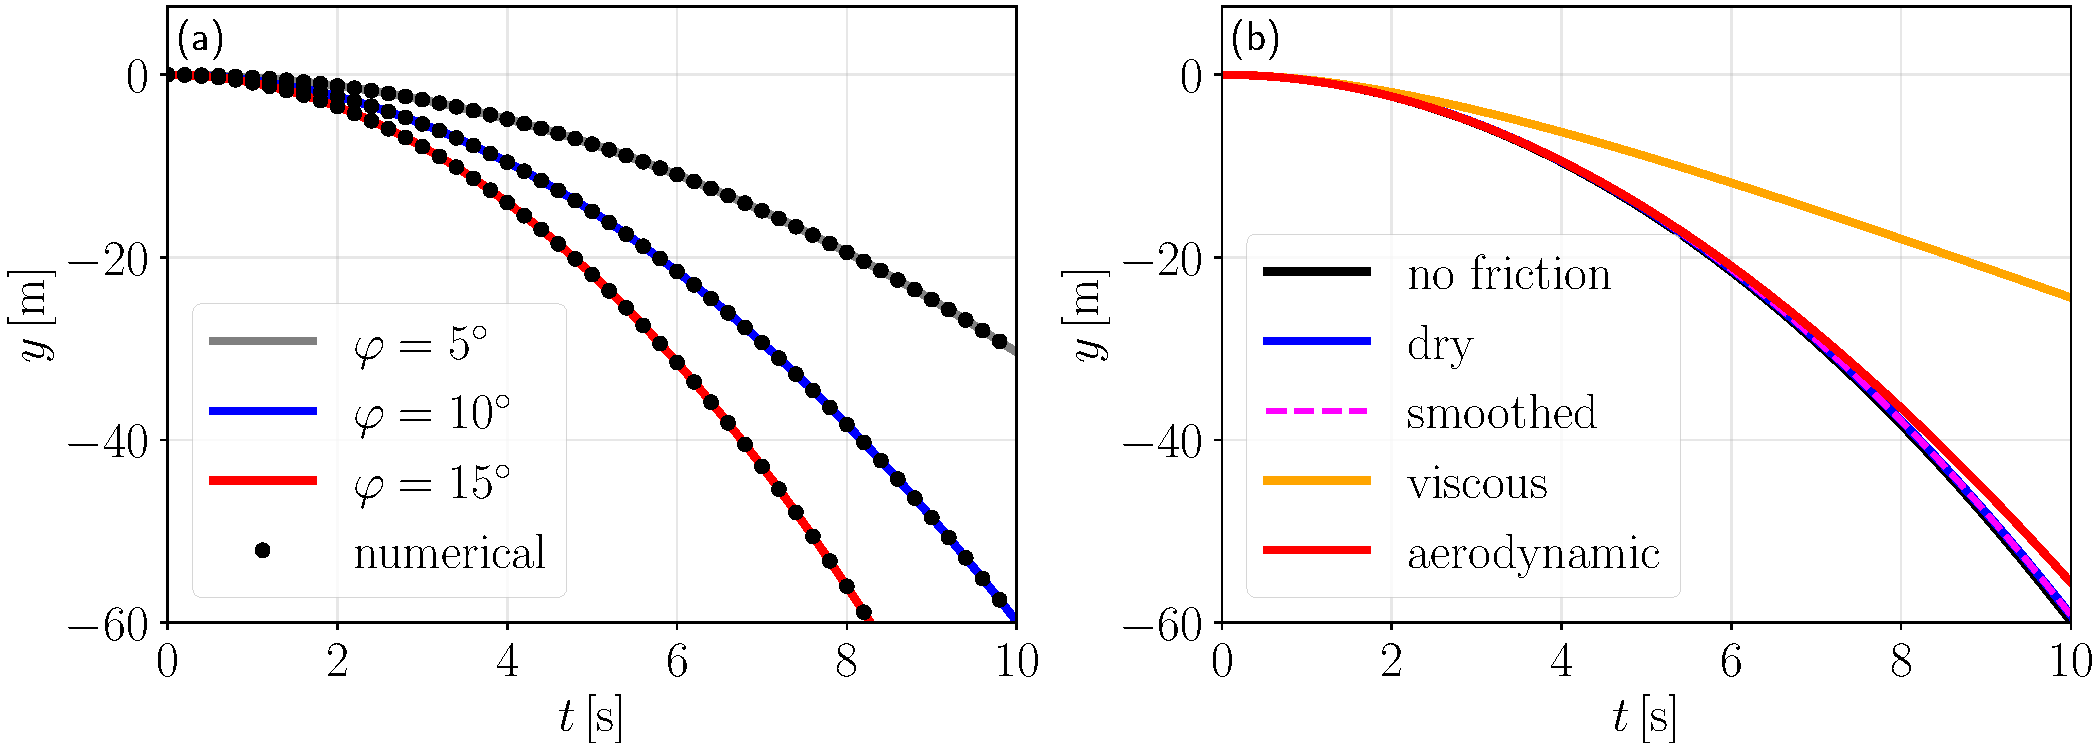
\includegraphics[width=\textwidth]{a.pdf}
    \caption{Numerical and analytical trajectories for different incline angles (a) and numerical trajectories for different kinds of friction (b). Fig. (a) shows no noticeable deviation between numerical and analytical values. Fig. (b) shows that the difference between discontinuous dry Coulomb friction and a smoothed variant are minimal, as is the general influence of this friction compared to no friction. Aerodynamic and viscous friction cause notable discrepancies.}
    \label{fig:a}
\end{figure}
As shown, the simulation agrees closely with the analytical solution. The maximal discrepancy between analytical and numerical values is $60.8 \, \unit{\micro\metre}$ for $\varphi = 5^\circ$, $120 \, \unit{\micro\metre}$ for $\varphi=10^\circ$, and $175 \, \unit{\micro\metre}$ for $\varphi=15 ^\circ$, thus not exceeding the micrometer scale. The remarkable discrepancy of the viscous approximation let us to discard this approach, while the smoothed Coulomb friction seemed sufficient to approximate the discontinuous dry friction. The almost negligible influence of Coulomb friction is in accordance with theoretical predictions in the case of ideal rolling without slipping.